% !TEX root = ../thesis.tex

\chapter{Implementierung}
\label{ch:implementierung}

\section{Aufbau}
\label{sec:aufbau}


\section{Interaktion und Parametrisierung}
\label{sec:interaktion}

Die Interaktion zwischen Mikado und dem Rekonstruktionstool findet über \ac{ROS} statt.
Das Tool ist dabei ein \texttt{ros::Subscriber} auf das von Mikado veröffentlichte Topic \texttt{/point\_cloud}.
Bei Aufnahme einer neuen Punktwolke wird somit das Durchlaufen der Pipeline automatisch angestoßen.

Weiterhin lassen sich über \texttt{rosparam set} und \texttt{rosparam get} Parameter setzen oder auslesen.
Diese werden dann im Programm geparst und - falls nicht vorhanden - durch Standardwerte ersetzt.
Dies bietet mehrere Vorteile gegenüber anderen Optionen:

\begin{itemize}
\item Parameter können optional über die Konsole, auf Programmebene oder auch gar nicht gesetzt werden.
\item Das Programm muss nicht für jede Konfiguration neu kompiliert werden und kann bei Laufzeit parametrisiert werden.
\item Die Interaktion mit anderen Programmen ist durch die Verwendung der \ac{ROS}-Schnittstelle erheblich vereinfacht.
\end{itemize}

Auch die Triangulation wird durch einen externen Trigger angestoßen.
Dieser wird als \texttt{rosservice} zur Verfügung gestellt, welcher mit dem Output-Dateipfad aufgerufen wird.
Auch hier ist durch die Verwendung der \ac{ROS}-basierten Schnittstelle eine hohe Flexibilität gegeben.


\section{Pipelineablauf}

\label{sec:pipeline}

\begin{figure}[ht]
    \centering
	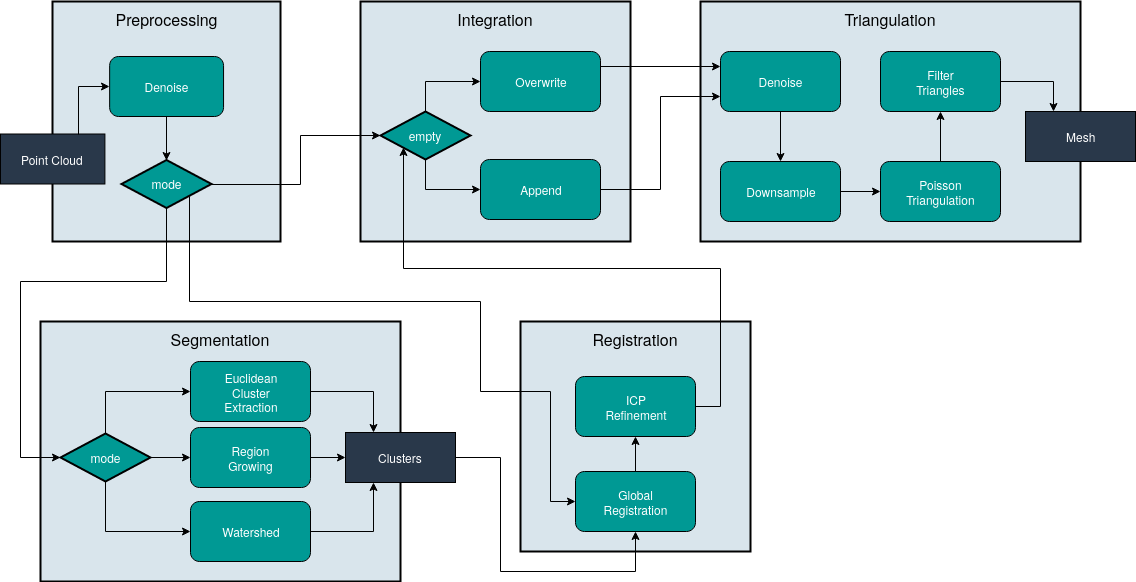
\includegraphics[width=\textwidth]{images/pipeline.png}
	\caption{Ablauf der Pipeline}
	\label{fig:pipeline}
\end{figure}

%TODO